%%%% Project report template for the course of Intelligent Agents 2026/2027
%%%% by Andrea Omicini <mailto:andrea.omicini@unibo.it>
%%%% after pikalab-unibo/report-template and unibo-fc-isi-ds/template-final-report
%%%%
%% Course strings live in course.sty, packages and the guidance environment in
%% style.sty. Put \templateguidanceoff below to drop every instruction at once.
\documentclass[11pt,a4paper]{scrartcl}
\usepackage{style}
%\templateguidanceoff
% version, read by the release job -- keep the three on separate lines
\newcommand{\versionmajor}{0}
\newcommand{\versionminor}{2}
\newcommand{\versionpatch}{0}
\newcommand{\version}{\versionmajor.\versionminor.\versionpatch}

\title{\LARGE
    Project Report Template\\
    (replace with the title of your project)
}
\subtitle{Project report for the course of \coursetitlelong{}, A.Y.\ \academicyear{} --- v.\ \version}

\author{
    Student 1 \\ \emailaddr{student1@studio.unibo.it}
    \and
    Student 2 \\ \emailaddr{student2@studio.unibo.it}
}

\date{\today}

\begin{document}

\maketitle

\begin{abstract}
    Up to $\sim$2000 characters stating what the project set out to do, how, and
    what came of it.
\end{abstract}

\section*{Disclaimer}

During the preparation of this work, the author(s) used [NAME THE TOOL OR
SERVICE] in order to [STATE WHAT FOR].
%
After using it, the author(s) reviewed and edited the content as needed, and
take(s) full responsibility for the content of this report and of the artefacts
it describes.

\begin{guidance}
Keep this section, filled in, if any tool or service --- generative or otherwise
--- contributed to the work or to the report. Delete it entirely if none did.
Declaring is not penalised; failing to declare is.
\end{guidance}

\begin{guidance}
\section*{How to use this template}

This is the report for the \emph{optional project} of \coursetitlelong{}
\academicyear{}. The project is worth up to 6/30, it assesses \emph{practical}
knowledge, it must cover or follow from a specific topic of the course, and it
must be agreed with the teacher beforehand --- see \url{\apiceprojects}.

A project may be \textbf{theoretical}, \textbf{technological} or
\textbf{methodological}, and the three do not fill this report in the same way:
%
\begin{itemize}
  \item every section carries a note saying what it expects from each kind;
  \item \Cref{sec:design,sec:implementation,sec:deployment} concern
  \emph{technological} projects, and should be dropped by the other two;
  \item a section that does not apply must be \emph{removed}, not left empty.
\end{itemize}

When the report is written, uncomment \texttt{\textbackslash
templateguidanceoff} in the preamble: every box like this one disappears, and
what is left is your report.
\end{guidance}

\begin{guidance}
\section*{Quick \LaTeX{} suggestions}

\begin{itemize}
  \item \textbf{Cite} with \texttt{\textbackslash cite}, giving the BibTeX key of
  an entry of \texttt{references.bib}, as in \cite{rao-agentspeak96}.
  Ready-made entries for most computer science papers are on
  \href{https://dblp.org/}{DBLP}; entries for the papers of the course are on
  \href{https://apice.unibo.it/}{APICe}.

  \item \textbf{Float} figures, tables and listings: put them in a
  \texttt{figure} or \texttt{lstlisting} environment and let \LaTeX{} place
  them. Do \emph{not} write placement hints such as \texttt{[h]} or
  \texttt{[h!]}. Label them, and reference the label with
  \texttt{\textbackslash cref} --- as in \cref{fig:universe} and
  \cref{lst:snippet} --- rather than writing ``the figure below''. Figures go
  in \texttt{figures/}, code in \texttt{listings/}.

  \item \textbf{Never break a line} with \texttt{\textbackslash\textbackslash}
  or \texttt{\textbackslash newline}. Leave a blank line to start a new
  paragraph; the indentation that follows is deliberate, and is how \LaTeX{}
  marks the paragraph break.

  \item \textbf{One sentence per source line}, with \texttt{\%} between the
  sentences of a paragraph, keeps diffs readable when the report is under
  version control.

  \item \textbf{Be consistent with notation}: $X$, X, $\mathbf{X}$,
  $\mathcal{X}$ and \texttt{X} are different symbols and should not denote the
  same thing.
\end{itemize}

\begin{figure}
    \centering
    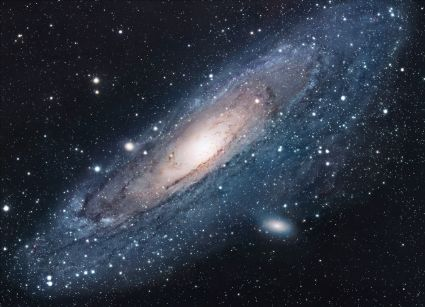
\includegraphics[width=0.5\linewidth]{figures/universe.jpg}
    \caption{An example figure.}
    \label{fig:universe}
\end{figure}

\javaimport[
    caption={An example listing.},
    label={lst:snippet}
]{listings/HelloWorld.java}
\end{guidance}

\section{Concept}
\label{sec:concept}

\begin{guidance}
\begin{itemize}
  \item Which \textbf{kind} of project is this --- theoretical, technological,
  methodological? Say so explicitly, in the first lines.

  \item Which \textbf{topic of the course} does it cover, or follow from?

  \item What is the project \emph{about}, in the terms of the course?
  \begin{itemize}
    \item for a \emph{theoretical} project: which question, thesis or model?
    \item for a \emph{technological} one: which artefact, and for whom?
    \item for a \emph{methodological} one: which practice, and whose?
  \end{itemize}

  \item Why is an \textbf{agent-oriented} reading the right one here? If the
  problem could be stated without agents, say why agents still earn their place
  --- or reconsider the project.

  \item What is deliberately \textbf{out of scope}?
\end{itemize}
\end{guidance}

\subsection{Objectives and definition of done}
\label{sec:objectives}

\begin{guidance}
\begin{itemize}
  \item State the objectives so that they can be \emph{checked}, and number
  them: they are referred to from \Cref{sec:validation}.

  \item Give each objective an \textbf{acceptance criterion} --- what would count
  as having met it, decided \emph{now} rather than after the fact.

  \item Which \textbf{artefacts} will be delivered? An argument, a model, a
  proof, a program, a corpus of experiments, a method, a guideline?

  \item If the project is a group one, who is responsible for what?
\end{itemize}
\end{guidance}

\section{Background and link to the course}
\label{sec:background}

\begin{guidance}
\begin{itemize}
  \item Which notions of \coursetitlelong{} does the project rest on? Be
  specific and cite: computational logic and logic programming, the BDI model
  of agency, coordination and interaction, the treatment of truth and knowledge
  in intelligent systems.

  \item What is the \textbf{state of the art} the project positions itself
  against, and what does the project add to it?

  \item Define the domain-specific terms you will use. A short glossary is
  welcome.

  \item This section is usually best written \emph{last}.
\end{itemize}
\end{guidance}

\section{Relevant agent and MAS features}
\label{sec:features}

\begin{guidance}
Argue which of the following are relevant to your project \emph{and which are
not} --- the exclusions matter as much as the inclusions, and a feature
dismissed with a reason is a sign the design was thought through. Whatever you
claim here is what \Cref{sec:contribution} must deliver on.

\begin{itemize}
  \item \textbf{autonomy and agency} --- in what sense is your entity an
  \emph{agent} rather than an object or a process? What does it decide by
  itself?

  \item \textbf{goal-directedness, and mental state} --- are beliefs, desires
  and intentions explicit in the model? Does the agent deliberate, or merely
  react?

  \item \textbf{reactivity and situatedness} --- what is the
  \emph{environment}? How does the agent perceive it and act upon it? Is the
  environment itself modelled as a first-class abstraction?

  \item \textbf{sociality, interaction and coordination} --- how many agents,
  and how do they interact? Which coordination model or medium --- message
  passing, tuple spaces, protocols? Who governs the interaction?

  \item \textbf{reasoning and inference} --- is reasoning symbolic, sub-symbolic
  or hybrid? Which logic, and why that one? What is decidable, and at what cost?

  \item \textbf{knowledge and truth} --- how is knowledge represented, and what
  is its epistemic status? What happens when beliefs turn out false, or when
  two agents disagree?

  \item \textbf{learning and adaptation} --- does anything change over time as a
  result of experience? Distinguish adaptation from mere configuration.

  \item \textbf{openness and heterogeneity} --- can agents join or leave? Are
  they built by different parties, on different technologies, with different
  interests?

  \item \textbf{organisation and norms} --- are there roles, institutions,
  obligations or prohibitions? What happens when a norm is violated?
\end{itemize}
\end{guidance}

\section{Contribution}
\label{sec:contribution}

\begin{guidance}
The core of the report.
%
A \emph{theoretical} project argues: definitions, model, claims, and the
reasoning that supports them.
%
A \emph{technological} project builds: fill in the two subsections below.
%
A \emph{methodological} project prescribes: the method, its steps, the
conditions under which it applies, and what it costs to follow.

Whatever the kind, report \textbf{why} each choice was made, against the
features claimed in \Cref{sec:features}. Alternatives considered and rejected
are worth reporting, with the reason.
\end{guidance}

\subsection{Design}
\label{sec:design}

\begin{guidance}
\emph{Technological projects.} Keep this technology-free as far as it will go:
the design should survive a change of language or framework.
%
\begin{itemize}
  \item \textbf{structure} --- which entities are modelled, and which of them
  are agents? Class diagrams, ontologies, the domain vocabulary.
  \item \textbf{interaction} --- protocols, sequence or activity diagrams, the
  coordination medium and its primitives.
  \item \textbf{behaviour} --- what each agent does: state diagrams, plan
  libraries, decision rules.
  \item \textbf{architecture} --- how the parts are organised into modules and
  distributed over nodes.
  \item \textbf{corner cases} --- failure detection, recovery, error reporting,
  graceful shutdown. What does an agent do when the environment lies to it?
\end{itemize}
\end{guidance}

\subsection{Implementation}
\label{sec:implementation}

\begin{guidance}
\emph{Technological projects.} Only what is interesting or non-trivial --- the
points where the design met resistance --- plus the technologies adopted and
why. Where generated documentation exists, reference it instead of repeating it.
\end{guidance}

\section{Validation}
\label{sec:validation}

\begin{guidance}
State the criterion \emph{before} the evidence, and tie it back to the numbered
objectives of \Cref{sec:objectives}.
%
\begin{itemize}
  \item \emph{theoretical} --- the proofs, or the arguments and the objections
  they answer. Which claims remain conjectural?
  \item \emph{technological} --- tests and their rationale: what was tested,
  how it was automated, how to run it, and which objective each test speaks to.
  Report how many pass of how many, and cover the corner cases.
  \item \emph{methodological} --- the case the method was applied to, and what
  applying it actually showed.
\end{itemize}

An honest negative result, explained, is worth more than a claim the evidence
does not support.
\end{guidance}

\section{Deployment and usage}
\label{sec:deployment}

\begin{guidance}
\emph{Technological projects only --- delete this section otherwise.}
%
How to install and launch the software on a machine with nothing on it: every
prerequisite with its version, every configuration step, and the expected
outcome of each. Then show it in use, with at least one worked example per
scenario.
\end{guidance}

\section{Self-evaluation}
\label{sec:selfevaluation}

\begin{guidance}
\emph{Group projects only --- for an individual project, a short paragraph is
enough.}
%
One subsection per member. Each member describes their own role and contribution
as objectively as they can, and assesses the strengths and the weaknesses of the
result. Each member is responsible only for their own subsection.
\end{guidance}

\section{Conclusions}
\label{sec:conclusions}

\begin{guidance}
What was done, what was not done and why, and what you learned --- including
what you would do differently.
\end{guidance}

\section{Future works}
\label{sec:futureworks}

\begin{guidance}
Where this would go next, concretely: the actual next step, not a wish list.
Anything left unimplemented belongs here, together with how you would have done
it.
\end{guidance}

\bibliographystyle{plain}
\bibliography{references}

\end{document}
